\chapter{Les structures arborescentes}
\minitoc
Nous allons voir deux types d'arbres : 
\begin{enumerate}
	\item L'arbre GRD : << Gauche Racine Droite >>
	\item Les arbres rouges noirs
\end{enumerate}
Ce sont des arbres binaires: chaque noeud de l'arbre à au lu deux fils. 
\attention{Les informations sont rangés dans l'arbre en respectant un certain critère}
\section{L'arbre GRD : <<Gauche Racine Droite>>}
	\subsection{Critère de rangement}
	Quelque soit le noeud de l'arbre : 
	\begin{itemize}
		\item les informations rangées à gauche de la racine de ce noeud sont inférieur ou égal à cette racine.
		\item les informations rangées à droite de la racine de ce noeud sont supérieur à cette racine.
	\end{itemize}
\begin{figure}[H]
\centering
\includegraphics[width=6cm]{content/schemas/arbresGRB.eps}
\caption{Arbre GRB}
\end{figure}
Cet arbre est prévu pour effectuer un parcours en profondeur.
	\subsection{Implémentation du TAD}
\begin{figure}[H]
\centering
\includegraphics[width=10cm]{content/schemas/arbresGRBImplementation.eps}
\caption{Implémentation de l'arbre GRB}
\end{figure}
\lstinputlisting[language=C, caption=Arbre GRD -- Header]{content/code/arbreGRB.h}
\lstinputlisting[language=C, caption=Arbre GRD -- Implémentation]{content/code/arbreGRB.c}

\subsection{Différents types de parcours}
\begin{description}
	\item[Parcours infixe] On parcours à gauche, on appel la valeur, on parcours à droite.
	\item[Parcours préfixe] On parcours on appel la valeur puis on parcours à gauche et à droite.
	\item[Parcours postfixe] On parcours à droite puis à droite et ensuite on appel la valeur.
\end{description}
\subsubsection{Exercices de parcours}
Écrire une fonction qui permette l'affichage en profondeur d'un arbre GRD mais sans utiliser la récursivité.\\
Nous avons utilisé une Pile afin de simuler des appels récursifs (Pile système). La pile contient le n\oe{}ud courant.

On suppose que l'on dispose du TAD \texttt{Pile} d'\texttt{Element} avec le type élément qui est une \texttt{Cel}.
\lstinputlisting[language=C, caption=Arbre GRD -- Implémentation fonction affichage en profondeur itératif]{content/code/arbreGRB-1.c}

Pour parcourir l'arbre en largeur, le principe est le même, à la place d'utiliser une \texttt{Pile} nous allons utiliser une \texttt{File}.
\lstinputlisting[language=C, caption=Arbre GRD -- Implémentation fonction affichage en longueur]{content/code/arbreGRB-2.c}

\subsection{Hauteur}
Si on considère $h$ la hauteur d'un arbre\footnote{La hauteur d'un arbre est la distance entre la racine et les feuilles}, la complexité des fonctions d'ajout et de recherche d'un arbre sont de complexité $O(h)$, $h$ doit donc être le plus petit possible.  

Pour cela, l'arbre doit être le plus équilibré possible pour cela, nous pouvons utiliser un arbre rouge-noir.

\section{Les arbres rouges noirs}
Cet arbre est presque équilibre, il comporte plusieurs propriétés.
\begin{enumerate}
	\item Par convention, un arbre vide est \textbf{noir}
	\item Les fils d'un nœud rouge sont \textbf{noirs}
	\item Le nombre de nœud noirs le long d'une branche dans l'arbre est indépendant de la branche 
\end{enumerate}

Le problème principal est donc de maintenir l'arbre rouge-noir.

\begin{figure}[H]
	\centering
	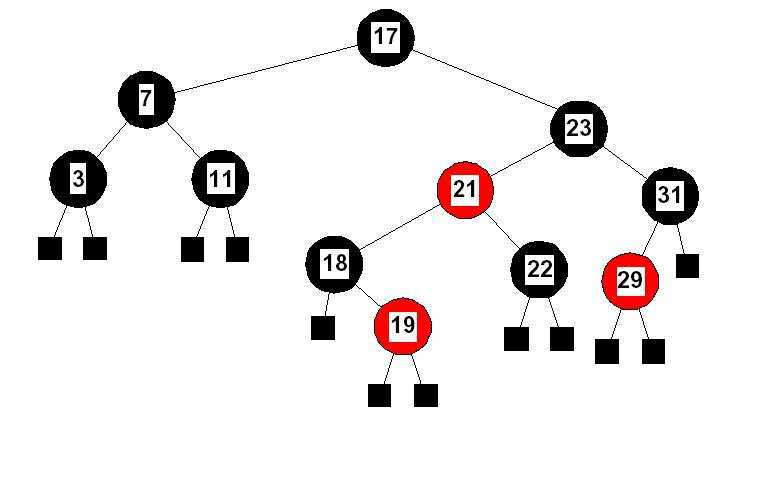
\includegraphics[width=10cm]{content/schemas/arbreRN.png}
	\caption{Exemple d'un arbre Rouge-Noir}
	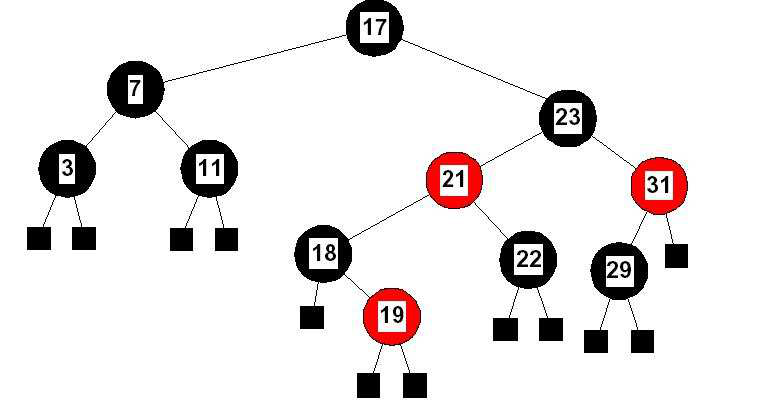
\includegraphics[width=10cm]{content/schemas/arbreNonRN.png}
	\caption{Exemple d'un arbre non Rouge-Noir}
\end{figure}
\subsection{Utilisation de rotation}
\begin{figure}[H]
	\centering
	\includegraphics[width=12cm]{content/schemas/arbresRotation.eps}
	\caption{Principe de la rotation}
\end{figure}
\attention{Les arbres rouges noirs sont des arbres GRD particuliers, ils possèdent donc les propriétés de l'arbre GRD}

\subsection{Ajout d'une valeur dans un arbre rouge-noir}
La valeur ajouté sera mise dans un noeud rouge dont les fils sont vies (donc noirs) avec une instruction classique dans l'arbre (comme un arbre GRD)

Plusieurs cas sont possibles:
\begin{itemize}
	\item C'est le 1\ier noeud de l'arbre $\Rightarrow$ rien à faire
	\item Son père est noir $\Rightarrow$ rien à faire
	\item Son père est rouge $\Rightarrow$ plusieurs sous cas.
		\begin{enumerate}
			\item Le père est la racine de l'arbre $\Rightarrow$ la racine devient noire
\begin{figure}[H]
	\centering
	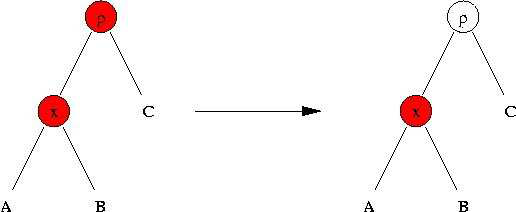
\includegraphics[width=7cm]{content/schemas/arbreRNcas0.png}
	\caption{Le père est la racine de l'arbre}
\end{figure}
			\item Le frère du père est rouge $\Rightarrow$ Alors le frère du père et le père passe noir et le grand-père devient rouge et on propage
\begin{figure}[H]
	\centering
	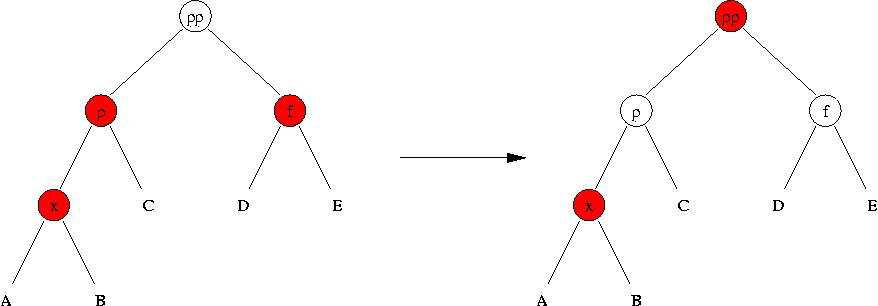
\includegraphics[width=12.5cm]{content/schemas/arbreRNcas1.png}
	\caption{Le frère du père est rouge}
\end{figure}
			\item Le frère f de p est noir 
				\begin{enumerate}
					\item[a.] x est le fils gauche de p 
\begin{figure}[H]
	\centering
	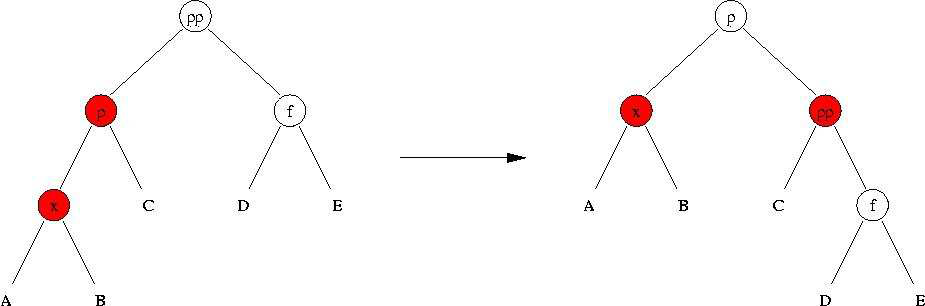
\includegraphics[width=12.5cm]{content/schemas/arbreRNcas2a.png}
	\caption{x est le fils gauche de p}
\end{figure}
					\item[b.] x est le fils droit de p 
\begin{figure}[H]
	\centering
	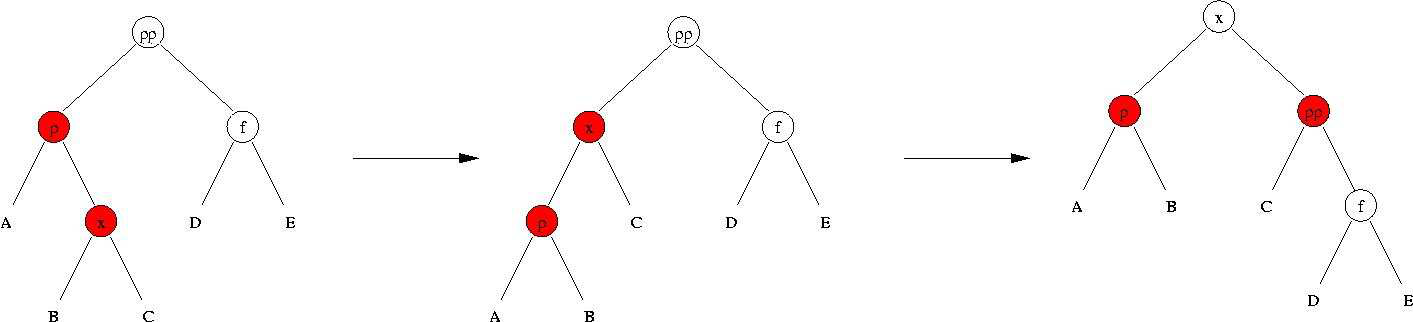
\includegraphics[width=12.5cm]{content/schemas/arbreRNcas2b.png}
	\caption{x est le fils droit de p}
\end{figure}
				\end{enumerate}
		\end{enumerate}
		\remarque{La seule propagation se fait dans le cas 1 (pas de propagation dans le cas 2}
\end{itemize}
\lstinputlisting[language=C, caption=Arbre GRD -- Implémentation]{content/code/arbreRougeNoir.c}
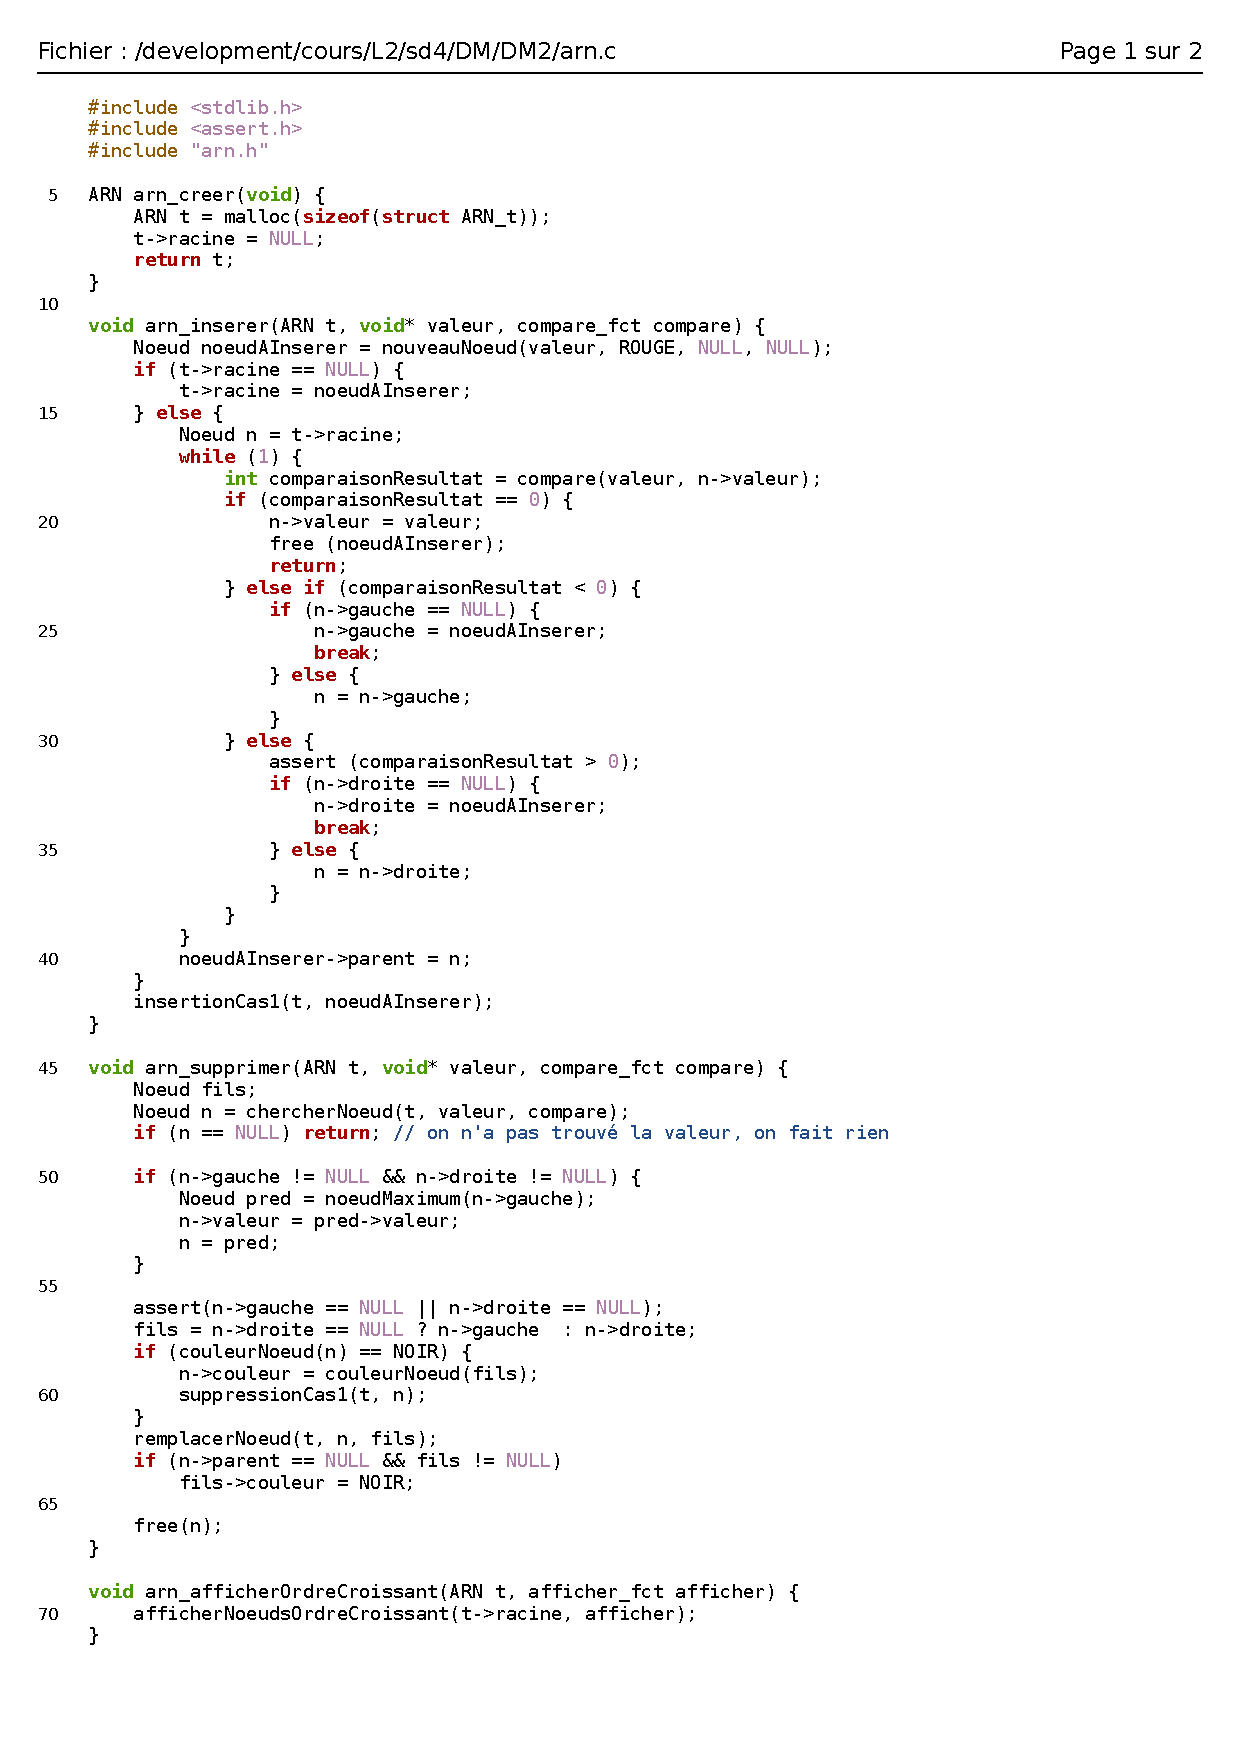
\includepdf[pages=1-]{arn.pdf}
